\documentclass[conference]{IEEEtran}

\usepackage{cite}
\usepackage{graphicx}
\usepackage{amsmath}
\usepackage{tabularx}
\usepackage{url}
\usepackage[hidelinks,breaklinks=true]{hyperref}

\graphicspath{{figures/}}
\hyphenation{furuta}

\begin{document}

\title{Rotary Inverted Pendulum: Comparison of Simulation and Physical Behaviour}

\author{
\IEEEauthorblockN{Henry Johnson}
\IEEEauthorblockA{
MEng Electrical and Electronic Engineering\\
University of Lincoln\\
School of Engineering\\
\texttt{25590191@students.lincoln.ac.uk}
}
}

\maketitle

\begin{abstract}
This report presents the design, simulation and practical evaluation of a rotary inverted pendulum, also referred to as a Furuta pendulum. The project combined a 3D-printed mechanical rig, Arduino-based embedded control and a nonlinear simulation model in order to compare expected behaviour with the response observed on the physical hardware. The simulation captured the dominant coupled dynamics of the rotary arm and pendulum link and was used as a reference for balance-controller assessment near the unstable upright equilibrium. With the current $125~\mathrm{mm}$ arm, the simulation predicts successful local recovery from an $8^\circ$ disturbance with modest control effort, whereas the physical build remains limited by stepper skipped steps, quantised actuation and the lack of direct arm-angle feedback. The results therefore show not only how the pendulum should behave in theory, but also why the practical rig does not yet match that ideal response.
\end{abstract}

\section{Introduction}
The rotary inverted pendulum is a well-established benchmark system in control engineering because it combines nonlinear dynamics, open-loop instability and underactuation in a single laboratory platform. Unlike a conventional cart-pole arrangement, the actuator in a Furuta pendulum applies torque to a horizontal rotating arm, while the pendulum itself is free to move in a vertical plane. This makes the system compact and mechanically attractive, but it also introduces strong dynamic coupling between the actuated and unactuated coordinates.

From a modelling perspective, the reverse pendulum is a useful example because small errors in the assumed inertia, damping or angle convention can lead to noticeably different simulated behaviour. For that reason, building a reliable simulation is not just a preliminary step before controller design; it is also a way of checking whether the physical assumptions are reasonable and whether the expected dynamic trends are present.

The aim of this work was not only to model the rotary inverted pendulum, but to compare the predicted behaviour with the behaviour of the real rig built for the coursework. The report therefore focuses on the physical system, the control approach, the simulation used as a reference, and the practical differences observed when the same ideas were transferred to hardware.

\section{Applications of the Rotary Inverted Pendulum}
Although the rotary inverted pendulum is often used as a teaching demonstrator, it is also a genuinely useful engineering benchmark. The system is underactuated, nonlinear and unstable around the operating point of interest, which means it exposes many of the same challenges that appear in larger electromechanical systems but in a more controlled laboratory form.

One important application is control-system education and validation. The rig can be used to demonstrate the difference between open-loop and closed-loop behaviour, the need for state estimation, and the practical limitations of linear control when the plant is strongly nonlinear. It is therefore well suited to modules covering classical control, state-space design, LQR, energy methods and embedded implementation.

The system is also relevant to robotics and mechatronics research. Many robotic platforms, including balancing robots, walking machines and lightweight manipulators, contain underactuated dynamics or unstable transient states. The Furuta pendulum provides a compact way to test strategies for stabilisation, switching control and disturbance rejection before similar ideas are applied to more expensive platforms.

In addition, the rig is useful as an actuator and sensing testbed. Because the pendulum reacts quickly to poor tuning, backlash, delay or missed motion, it becomes an effective way to evaluate whether a chosen motor, driver and encoder arrangement is genuinely suitable for closed-loop control. In this project that aspect became especially important because the use of a stepper motor introduced skipped-step behaviour that would not be apparent in a purely static test.

\section{Hardware Design and Fabrication}
\subsection{Mechanical Design}
The physical rig was designed specifically around the selected stepper motor and incremental encoder rather than being assembled from generic laboratory brackets. The horizontal carrier arm was set to $125~\mathrm{mm}$ in length, while the pendulum assembly had an overall vertical height of approximately $280~\mathrm{mm}$. The pendulum top hub was designed with an $18~\mathrm{mm}$ outer diameter, a $14~\mathrm{mm}$ axial length and a $6~\mathrm{mm}$ bore so that it could clamp directly to the encoder interface.

The printed parts were manufactured on Bambu printers, which made it practical to iterate the geometry quickly and produce parts that matched the motor and encoder mounting constraints. This was useful because the project required more than a simple pendulum rod: the fixtures needed to position the encoder accurately, support the motor-side arm and protect the Arduino hardware in a compact footprint.

The main CAD artefacts prepared for the build are stored in \path{report/design/} and were:
\begin{itemize}
\item \path{pendulum.stl}, representing the pendulum-side geometry;
\item \path{motor loop.stl}, representing the motor-side arm or carrier feature;
\item \path{arduino_box_with_roof.stl}, representing the electronics housing.
\end{itemize}

These files are intended to be uploaded to the project GitHub repository alongside the control code so that the mechanical and electrical design can be reproduced.

\subsection{Electrical Hardware}
The control hardware was based on an Arduino Uno Rev3 fitted with an Arduino Motor Shield Rev3. Actuation was provided by a 42BYGH162-A-21DH stepper motor and sensing by an E38S6G5-600B-G24N incremental encoder. In the present build, the encoder was used to measure pendulum angle directly, while the rotary arm angle was estimated in software from the number of commanded stepper steps. Because the Motor Shield already occupies one of the standard interrupt-capable pins, the current Arduino sketch decodes channel-A transitions only, giving $1200$ usable edge counts per revolution from the nominal $600$ pulse encoder rather than full $4\times$ quadrature decoding. This decision allowed the system to be implemented with the available hardware, but it also introduced an important limitation because the arm angle estimate remains correct only while the motor follows every commanded step.

\begin{figure}[!t]
\centering
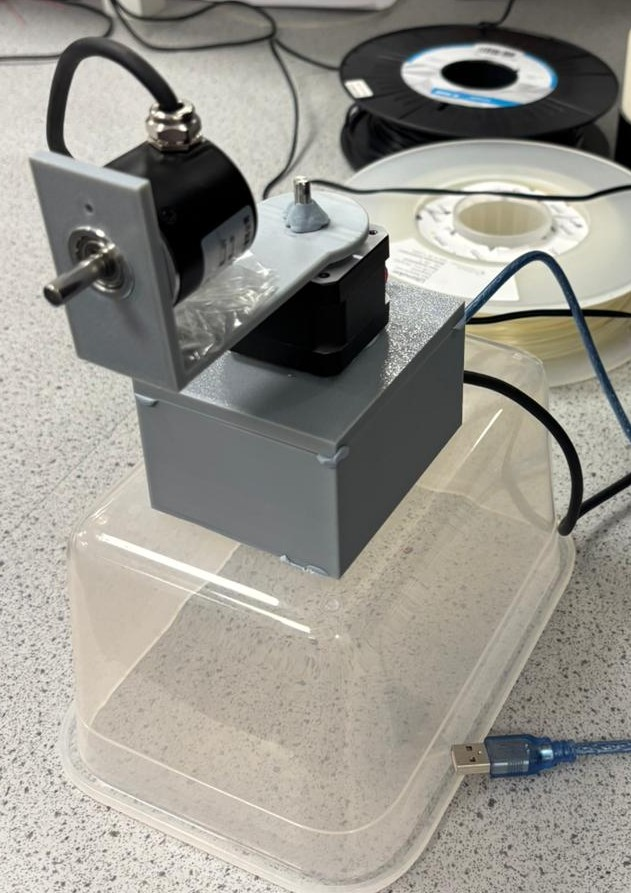
\includegraphics[width=\columnwidth]{system.jpeg}
\caption{Full Hardware Implementation of the Rotary Inverted Pendulum.}
\label{fig:hardware_placeholder}
\end{figure}

\subsection{Sensor and Actuator Comparison}
The selected sensor and actuator were adequate for building a first working prototype, but they were not necessarily the optimum choices for high-performance closed-loop balancing. Table~\ref{tab:hardware_compare} summarises the chosen components against realistic alternatives.

\begin{table}[!t]
\centering
\caption{Short comparison of the selected sensor and actuator against alternatives}
\label{tab:hardware_compare}
\scriptsize
\renewcommand{\arraystretch}{1.12}
\begin{tabularx}{\columnwidth}{|p{1.1cm}|p{2.15cm}|X|}
\hline
Role & Chosen hardware & Critical comment \\
\hline
Sensor & Incremental encoder & Better repeatability and continuous rotation than a potentiometer, but unlike an absolute magnetic encoder it needs decoding and start-up calibration. \\
\hline
Actuator & Bipolar stepper motor & Easy to command and mount, but it can skip steps under aggressive motion and is weaker than a geared DC motor with encoder or a servo-class actuator. \\
\hline
Drive & Arduino Motor Shield Rev3 & Convenient and available, but not optimised for stepper current control, so torque smoothness and higher-speed performance are limited compared with a dedicated stepper driver. \\
\hline
\end{tabularx}
\end{table}

\subsection{Practical Hardware Behaviour}
The most significant mismatch between the idealised design and the physical rig was skipped steps in the stepper motor. In the mathematical model, the arm input is treated as if the actuator follows the demanded motion exactly. In practice, if the stepper is asked to accelerate too quickly, if the torque demand exceeds the available motor torque, or if the power stage cannot supply current cleanly enough, the motor can miss steps. Once this happens, the internally estimated arm angle drifts away from the real arm position, and the controller is no longer regulating the state it believes it is regulating.

This behaviour can be reduced in several ways. The first is to use conservative acceleration ramps and step-rate limits, which has been built into the final Arduino sketch. The second is to reduce the mechanical load by lowering inertia, reducing friction and ensuring good alignment of the printed parts. The third is to improve the actuation chain, for example by replacing the L298-based shield with a dedicated stepper driver with current control, or by using a geared DC motor or servo arrangement more suited to continuous closed-loop position control. Finally, the most robust improvement would be to measure the arm angle directly with either a second encoder or a homing/reference mechanism so that missed steps can be detected and corrected.

\section{Rotary Inverted Pendulum Model}
\subsection{System Description}
The model uses two generalised coordinates. The first coordinate, $\theta$, is the angular position of the rotary arm about the vertical axis. The second coordinate, $\alpha$, is the pendulum angle measured relative to the upright position. With this convention, $\alpha = 0$ corresponds to the unstable equilibrium that the controller must regulate.

The state vector is written as
\begin{equation}
x =
\begin{bmatrix}
\theta & \alpha & \dot{\theta} & \dot{\alpha}
\end{bmatrix}^{T}.
\end{equation}

The actuator torque is applied only to the arm, which means the system has fewer control inputs than degrees of freedom. This underactuated structure is the main reason the pendulum is difficult to stabilise and why the simulation is an important design tool.

\subsection{Modelling Assumptions}
To keep the simulation model practical while preserving the dominant physics, the following assumptions are used:
\begin{itemize}
\item The arm and pendulum are treated as rigid bodies.
\item The pendulum motion is confined to a single vertical plane attached to the rotating arm.
\item Joint friction is represented using lumped viscous damping terms.
\item The actuator is represented as an equivalent input torque applied directly to the rotary arm.
\item Structural flexibility, backlash and sensor quantisation are neglected in the first instance.
\end{itemize}

These assumptions are reasonable for an initial nonlinear simulation and help keep the model transparent enough to tune, validate and linearise later if required.

\subsection{Nonlinear Dynamic Form}
The equations of motion can be expressed in the standard manipulator form
\begin{equation}
M(q)\ddot{q} + C(q,\dot{q})\dot{q} + D\dot{q} + G(q) =
\begin{bmatrix}
\tau \\
0
\end{bmatrix},
\label{eq:manipulator}
\end{equation}
where
\begin{equation}
q =
\begin{bmatrix}
\theta \\
\alpha
\end{bmatrix}.
\end{equation}

In (\ref{eq:manipulator}), $M(q)$ is the configuration-dependent inertia matrix, $C(q,\dot{q})\dot{q}$ contains the Coriolis and centrifugal effects, $D\dot{q}$ represents viscous damping, $G(q)$ is the gravity vector, and $\tau$ is the motor torque applied to the arm. Since the pendulum joint is unactuated, the second input term is zero.

This formulation is particularly useful because it separates the model into physically meaningful contributions. In practice, the dynamics function can evaluate these terms for the current state and then solve for $\ddot{q}$, allowing the complete state derivative $\dot{x}$ to be returned to the numerical integrator.

\subsection{Linearised Interpretation}
Although the simulation itself is nonlinear, it is still helpful to view the plant locally around the upright equilibrium. For small perturbations about $\alpha = 0$, the model can be linearised into the form
\begin{equation}
\delta\dot{x} = A\delta x + B\delta u.
\end{equation}

This local representation is useful when moving toward classical or modern control design, for example PD, state feedback or LQR methods. However, the full nonlinear model remains the more informative representation when studying large-angle excursions, swing-up behaviour or sensitivity to initial condition.

\section{Closed-Loop Control System Design}
\subsection{Balance Controller}
The closed-loop balancing controller was designed around the upright operating point, where $\alpha = 0$. In this region the nonlinear model can be linearised and treated as a four-state system using the state vector
\begin{equation}
x =
\begin{bmatrix}
\theta & \alpha & \dot{\theta} & \dot{\alpha}
\end{bmatrix}^{T}.
\end{equation}

The stabilising feedback law is written in the standard state-feedback form
\begin{equation}
u_{b} = -Kx,
\end{equation}
where $u_{b}$ is the commanded arm action and $K$ is the gain vector. In the simulation workflow, the linearised plant is obtained numerically and a stabilising gain set is generated for the local model. The purpose of this controller is not to swing the pendulum up from the hanging position, but to capture and regulate it once it enters a sufficiently small region around upright.

In the Arduino implementation, the same idea is preserved in embedded form. The measured or estimated states are combined to produce a normalised command, with pendulum angle and pendulum angular rate weighted most heavily because they dominate the local stability problem. The arm angle and arm angular rate are also included so that the controller does not stabilise the pendulum at the expense of uncontrolled arm rotation.

\subsection{Swing-Up Controller}
Because the upright equilibrium is unstable, the balancing controller alone is not enough to recover the system from the hanging configuration. For that reason, the Arduino controller also includes an energy-based swing-up mode. The idea is to inject energy into the pendulum gradually until the total energy approaches the amount required for the upright state.

The swing-up energy measure can be written as
\begin{equation}
E = \frac{1}{2}J_{eq}\dot{\alpha}^{2} + m_{p}gl_{p}(1+\cos\alpha),
\end{equation}
where $J_{eq}$ is the effective pendulum inertia about the pivot. With this definition, the hanging position has low energy and the upright position corresponds to the desired energy target
\begin{equation}
E_{d} = 2m_{p}gl_{p}.
\end{equation}

The implemented swing-up law uses the energy difference together with the pendulum motion direction to decide whether the arm should add or remove energy. A practical form of the command is
\begin{equation}
u_{s} = k_{E}(E_{d} - E)\,\mathrm{sgn}(\dot{\alpha}\cos\alpha)
        - k_{\theta}\theta - k_{\dot{\theta}}\dot{\theta},
\end{equation}
where the additional arm-angle and arm-rate terms stop the arm from drifting too far while the energy is being pumped into the pendulum. Once the pendulum enters a capture region close to upright, the controller switches from swing-up mode to balancing mode.

\subsection{Mode Switching and Stepper Command Shaping}
The Arduino sketch therefore operates as a switched controller with two modes:
\begin{itemize}
\item an energy-based swing-up mode for large pendulum excursions;
\item a local state-feedback balance mode when the pendulum is sufficiently close to upright.
\end{itemize}

The switching threshold in the embedded code is based on pendulum angle and angular rate. A representative capture rule is to enter balance mode only when the pendulum is within a small angular window around upright and the angular rate is low enough that the balancing controller can take over safely.

Because the actuator is a stepper motor driven through an H-bridge shield, the control signal cannot be applied as an ideal continuous torque. Instead, the embedded controller converts the normalised command into a demanded step rate and then applies an acceleration-limited ramp before issuing actual full steps. This is an important practical detail because abrupt commands increase the risk of missed steps, which would otherwise corrupt the estimated arm angle. The final code in \texttt{arduino/arduino.ino} therefore includes explicit step-rate limiting, acceleration limiting, swing-up logic, balance logic and serial calibration commands.

\section{Simulation Method and Parameterisation}
\subsection{Simulation Workflow}
The simulation is organised around a main driver script and a dedicated dynamics function. In this workflow, \texttt{furuta\_main.m} is responsible for defining the parameter set, estimating mass properties from the measured geometry, linearising the plant numerically, synthesising the stabilising state feedback law, solving the response and exporting the figures used in this report. The companion file \texttt{furuta\_dynamics.m} evaluates the nonlinear equations of motion for the current state.

This separation is good practice because it keeps the physics of the model independent from the plotting and simulation configuration. It also makes the code easier to debug. If the predicted response looks unrealistic, the numerical setup and the physical model can be checked independently instead of being mixed together in a single script.

A typical simulation sequence is:
\begin{enumerate}
\item define the physical parameters and initial state;
\item call the numerical solver over the required time interval;
\item recover the arm angle, pendulum angle and angular velocities;
\item generate plots for interpretation and comparison.
\end{enumerate}

\subsection{Simulation Parameters}
The final simulation model was parameterised directly from the supplied arm, hub and pendulum dimensions. Where mass properties were not measured experimentally, they were estimated by assuming aluminium components with a density of $2700~\mathrm{kg/m^3}$ and by including a small additional inertia allowance at the motor side to account for the coupler and fixture. The resulting parameter set is listed in Table~\ref{tab:params}.

\begin{table}[!t]
\caption{Parameters used in the simulation reference model}
\label{tab:params}
\centering
\footnotesize
\begin{tabular}{|p{2.45cm}|c|c|}
\hline
Quantity & Symbol & Value \\
\hline
Arm length & $L_{r}$ & $0.125~\mathrm{m}$ \\
\hline
Pendulum rod length & $L_{rod}$ & $0.266~\mathrm{m}$ \\
\hline
Overall height & $L_{tot}$ & $0.280~\mathrm{m}$ \\
\hline
Estimated arm mass & $m_{r}$ & $0.0324~\mathrm{kg}$ \\
\hline
Pendulum mass & $m_{p}$ & $0.0373~\mathrm{kg}$ \\
\hline
Pendulum COM offset & $l_{p}$ & $0.1149~\mathrm{m}$ \\
\hline
Arm inertia & $J_{r}$ & $1.94\times10^{-4}~\mathrm{kg\,m^2}$ \\
\hline
Pendulum inertia & $J_{p}$ & $2.99\times10^{-4}~\mathrm{kg\,m^2}$ \\
\hline
Arm viscous damping & $b_{r}$ & $1.2\times10^{-3}~\mathrm{N\,m\,s/rad}$ \\
\hline
Pendulum damping & $b_{p}$ & $8.0\times10^{-4}~\mathrm{N\,m\,s/rad}$ \\
\hline
Gravitational acceleration & $g$ & $9.81~\mathrm{m/s^{2}}$ \\
\hline
Torque saturation & $\tau_{max}$ & $\pm0.18~\mathrm{N\,m}$ \\
\hline
Encoder resolution & -- & $600$ pulses/rev nominal \\
\hline
Initial pendulum angle & $\alpha(0)$ & $8^\circ$ \\
\hline
Simulation duration & $T$ & $2.5~\mathrm{s}$ \\
\hline
\end{tabular}
\end{table}

In the final implementation, the nonlinear model was integrated with \texttt{ode45}. The corresponding hardware platform used for practical comparison was an Arduino Uno Rev3 with a Motor Shield Rev3, a 42BYGH162-A-21DH motor and an E38S6G5-600B-G24N incremental encoder. Within the simulation, the motor-drive chain was approximated as a saturated torque source and the encoder resolution was retained as a hardware reference, rather than directly quantising the states at this stage.

\subsection{Role of the Simulation}
The purpose of the simulation in this project was to provide a reference against which the physical rig could be judged. It allowed the expected open-loop instability, local balance recovery and control-effort demand to be examined before comparing those predictions with the real system. This was especially useful because the practical rig introduced non-idealities, such as skipped steps and unmeasured arm-position drift, that are much easier to interpret once the underlying idealised behaviour is already understood.

\section{Comparison of Simulation and Physical Behaviour}
\subsection{Expected Dynamic Behaviour}
For a rotary inverted pendulum, the open-loop response near the upright equilibrium is expected to be unstable. Even a small perturbation in $\alpha$ should grow unless a stabilising control action is applied. The arm motion and pendulum motion are also expected to be strongly coupled, meaning that motion in one coordinate produces a noticeable response in the other.

If the model has been implemented consistently, the simulation should show the following qualitative features:
\begin{itemize}
\item rapid sensitivity to small initial disturbances around the upright position;
\item coupled exchange of energy between the rotary arm and pendulum link;
\item clear influence of damping on how aggressively the motion grows or decays;
\item strong dependence of the response on the chosen input torque or control law.
\end{itemize}

These are important checks because they help confirm that the model is behaving like an underactuated inverted pendulum rather than a loosely related two-link mechanism.

\subsection{Simulation Reference Response}
Figure~\ref{fig:model_placeholder} shows the geometry used to parameterise the model, while Fig.~\ref{fig:response_placeholder} compares the open-loop and closed-loop nonlinear responses for an initial pendulum disturbance of $8^\circ$ away from the upright equilibrium.

\begin{figure}[!t]
\centering
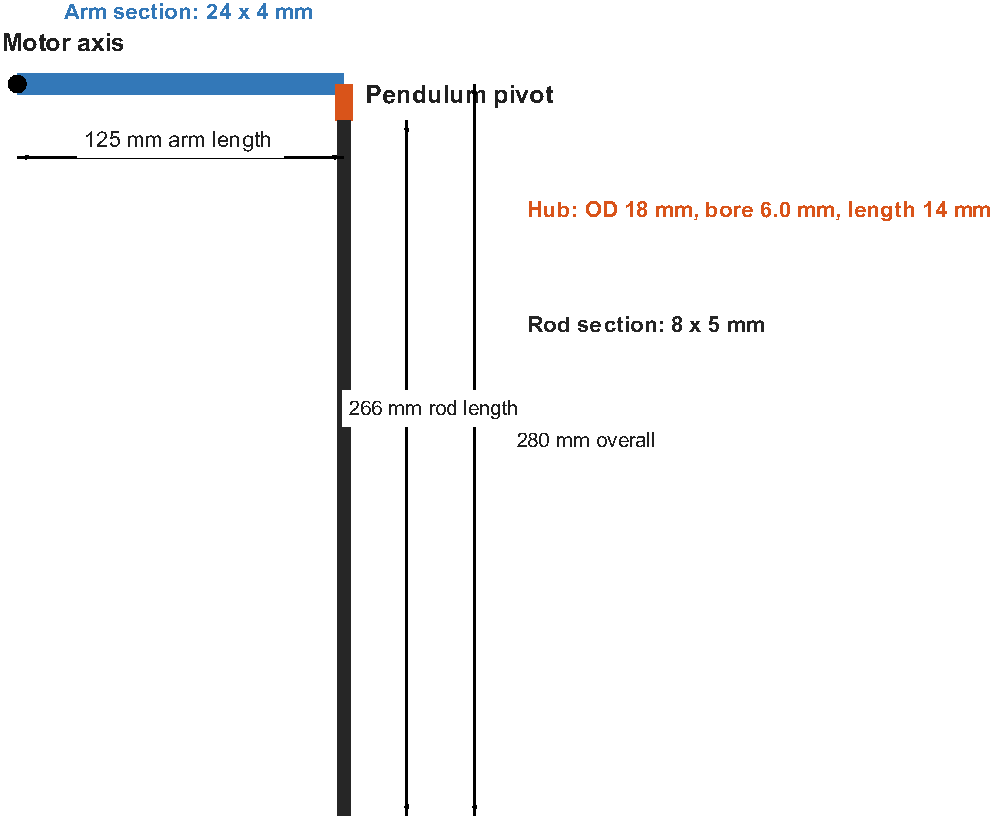
\includegraphics[width=\columnwidth]{furuta_geometry.pdf}
\caption{Geometry used to parameterise the simulation from the measured coursework dimensions.}
\label{fig:model_placeholder}
\end{figure}

\begin{figure*}[!t]
\centering
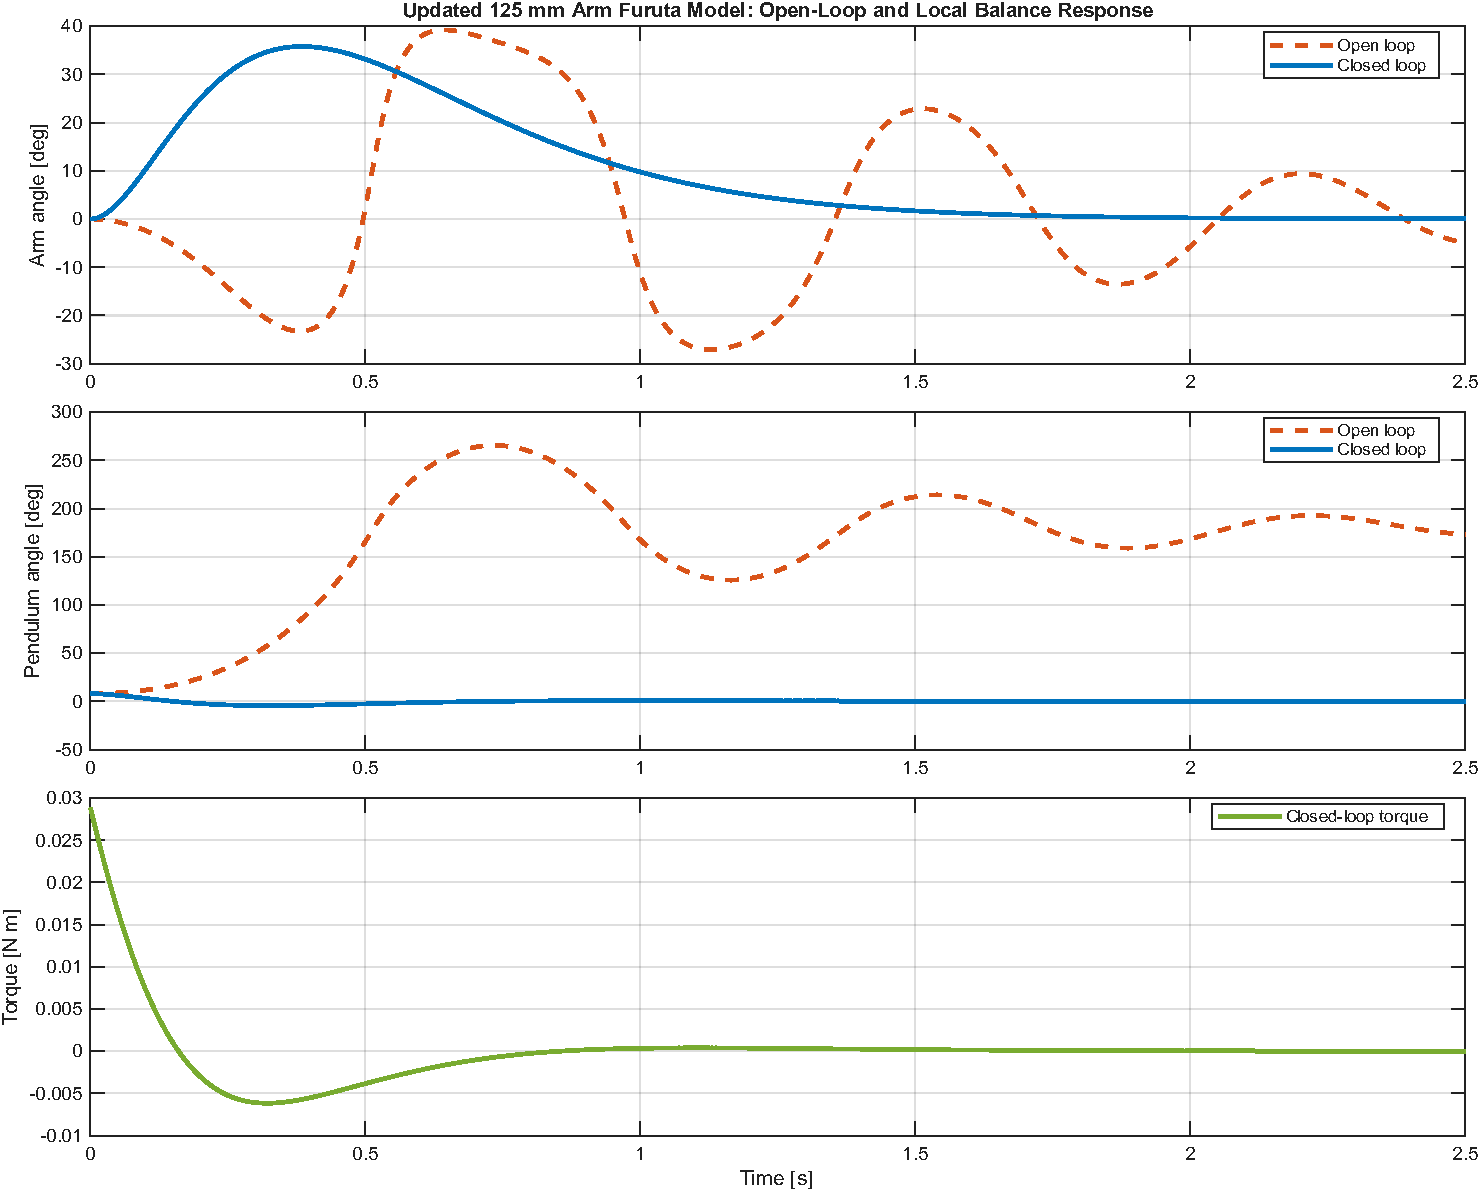
\includegraphics[width=0.95\textwidth]{furuta_response.pdf}
\caption{Nonlinear simulation of the rotary inverted pendulum, comparing open-loop and closed-loop behaviour for an initial pendulum disturbance of $8^\circ$.}
\label{fig:response_placeholder}
\end{figure*}

The simulation plots in Fig.~\ref{fig:response_placeholder} assess the local stabilising controller around the upright operating point. In other words, these plots are intended to show the balancing behaviour once the pendulum is already close enough to upright for local state feedback to be effective. The embedded Arduino implementation extends this by adding a separate swing-up mode for large-angle operation on the physical rig.

The open-loop response behaves as expected for an inverted system. Starting from a modest angular disturbance, the pendulum quickly departs from the unstable equilibrium and moves toward the hanging configuration. In the present simulation the pendulum angle progresses toward approximately $180^\circ$ within the first second, which is fully consistent with an unforced reverse pendulum.

The closed-loop response shows that the current $125~\mathrm{mm}$ arm geometry is favourable for local balancing. Starting from the same $8^\circ$ initial disturbance, the simulated pendulum returns to upright quickly and the control effort stays comfortably below the imposed torque limit. This is a useful result because it suggests that the selected arm length provides significantly better leverage over the pendulum, making the idealised plant locally controllable with the present balance gain set.

The main quantitative observations from the simulation are:
\begin{itemize}
\item settling time within $\pm 2^\circ$: approximately $0.540~\mathrm{s}$;
\item final closed-loop pendulum angle: approximately $0.009^\circ$;
\item peak arm excursion in closed loop: approximately $35.8^\circ$;
\item peak equivalent control torque: approximately $0.029~\mathrm{N\,m}$.
\end{itemize}

It is also worth noting that the simulated control torque remains well below the assumed saturation limit of $\pm 0.18~\mathrm{N\,m}$. This suggests that, for the updated geometry and initial condition used here, the idealised plant is no longer torque-limited in the same way as the earlier shorter-arm case. In practice, the real rig is still likely to exhibit larger losses than the idealised simulation because backlash, current limiting, encoder noise and stepper nonlinearity have not yet been modelled explicitly.

\subsection{Using the Simulation as a Hardware Reference}
One of the main strengths of the simulation is that it creates a bridge between theoretical control design and the practical hardware implementation. Before applying a controller to the physical rig, it is much safer to examine the predicted response and verify that the signs, angle conventions and parameter magnitudes are sensible.

This is particularly important for a reverse pendulum because the real platform can respond very quickly once the pendulum moves away from the upright position. A simulation therefore reduces development risk. It also helps identify whether later hardware problems are likely to come from the control law itself or from practical issues such as sensor noise, saturation, backlash or actuator delay that were not included in the initial model. In this project the most important practical discrepancy was stepper skipping. Even when the pendulum-side encoder behaved correctly, any lost motor steps caused the estimated arm state to diverge from the true arm state. This is one of the clearest reasons why a real build can fail even when the nonlinear model appears well behaved.

\subsection{Experimental Observations from the Hardware}
The most important experimental observation from the physical build was that the stepper-driven arm did not behave as ideally as the simulation assumed. During preliminary hardware trials, the motor was observed to skip steps during aggressive reversals and during high-demand portions of the motion, especially when the control action changed quickly. Once this occurred, the internally estimated arm angle no longer matched the real arm angle, and the quality of the balancing action degraded immediately.

The second observation was that the real hardware response was visibly less smooth than the simulated response. The simulation produces continuous state trajectories because the actuator is modelled as an idealised torque input. By contrast, the physical rig moves in a quantised and more abrupt way because the stepper is driven through discrete steps and the motor shield is not a true closed-loop current-regulated stepper driver. This introduces audible vibration, more noticeable transients around reversal points and higher sensitivity to friction and alignment.

The third observation was that controller performance on hardware was more sensitive to setup details than in the simulation. Small changes in cable routing, stiffness of the printed mounts, supply quality and arm alignment had a visible effect on behaviour. This is consistent with the expectation that the real system contains unmodelled friction, compliance and backlash.

\subsection{Direct Comparison Between Simulation and Physical Behaviour}
Table~\ref{tab:sim_vs_hardware} summarises the most important differences between the simulated plant and the physical build. This comparison is useful because it shows clearly that the main limitations are not in the mathematical structure of the Furuta model itself, but in the actuator realisation and the incomplete state feedback available on the current rig.

\begin{table*}[!t]
\centering
\caption{Comparison between simulated behaviour and physical hardware behaviour}
\label{tab:sim_vs_hardware}
{\footnotesize
\begin{tabular}{|p{2.55cm}|p{4.2cm}|p{4.5cm}|p{3.1cm}|}
\hline
Aspect & Simulation behaviour & Physical behaviour & Implication \\
\hline
Actuation model & Smooth equivalent torque input with no lost motion & Discrete stepper actuation through the motor shield, with observed skipped steps under aggressive motion & Real hardware is harder to stabilise than the idealised simulation suggests \\
\hline
Arm angle knowledge & Exact state available from the solver & Estimated from commanded steps only unless additional sensing is added & Step loss causes state-estimation drift \\
\hline
Closed-loop recovery near upright & The current $125~\mathrm{mm}$ arm model recovers from an $8^\circ$ disturbance in about $0.54~\mathrm{s}$ and remains close to upright afterwards & Recovery near upright was inconsistent on the physical rig and depended strongly on skipped steps, alignment and supply conditions. & The model now suggests the controller is adequate in principle, so the remaining gap is dominated by hardware limitations rather than lack of ideal control authority \\
\hline
Motion smoothness & Continuous and symmetric response curves & More vibration, harsher reversals and higher sensitivity to mechanical alignment & Strong evidence of actuator and structural non-idealities \\
\hline
Repeatability & Repeatable for fixed parameters and initial conditions & Repeatability across repeated hardware tests was inconsistent, with noticeable trial-to-trial variation in capture and stabilisation behaviour. & Indicates sensitivity to unmodelled actuator and mechanical effects \\
\hline
\end{tabular}
}
\end{table*}

\section{Critical Evaluation of the Selected Hardware}
The chosen encoder and stepper motor made it possible to realise a low-cost prototype using readily available parts, but the combination is better suited to demonstrating system concepts than to delivering robust high-performance control. The E38S6G5-600B-G24N incremental encoder is a reasonable pendulum-angle sensor because it provides repeatable angular increments and can rotate continuously. However, it is not an absolute sensor, so it requires calibration at start-up and does not, by itself, recover the true angle after a reset or disconnection. An absolute magnetic encoder would reduce that calibration burden and simplify start-up behaviour.

The more serious limitation lies on the actuator side. The 42BYGH162-A-21DH stepper motor is attractive because it is easy to source, easy to mount and easy to command in open loop. For a Furuta pendulum, however, the major disadvantage is that open-loop stepper positioning only remains trustworthy while every commanded step is physically achieved. The moment the motor misses steps, the arm-angle estimate becomes incorrect and the controller acts on the wrong state. A geared DC motor with an arm-side encoder, or a servo-class actuator with direct position feedback, would therefore be a stronger long-term choice for reliable closed-loop stabilisation.

The Arduino Motor Shield Rev3 is similarly convenient but not ideal. It provides an accessible route to early experimentation, yet it does not offer the same current regulation, microstepping capability or torque smoothness as a dedicated stepper driver. That means the final hardware performance is constrained not only by control tuning, but also by the power electronics. In critical terms, the selected hardware was sufficient for prototyping and demonstrating the control concepts, but it does not represent the most robust architecture for precision balancing or repeatable swing-up capture.

\subsection{Video, Source Code and Design Files}
\noindent\textbf{Video Evidence:} \href{https://youtube.com/shorts/5Z5avwsL-BM}{\nolinkurl{https://youtube.com/shorts/5Z5avwsL-BM}}. \par
\noindent\textbf{GitHub Repository:} \href{https://github.com/Thomriiii/Sensors-Actuators-Controllers/tree/main/Coursework2}{\nolinkurl{https://github.com/Thomriiii/Sensors-Actuators-Controllers/tree/main/Coursework2}}. \par
\section{Limitations and Future Development}
The present simulation model is useful for studying the principal dynamics of the system, but it still has practical limitations. In its current form, the model is unlikely to capture every non-ideal effect present in the real hardware. Motor saturation, dead-zone behaviour, structural compliance, encoder quantisation and Coulomb friction can all become significant when moving from simulation to experiment. The most significant missing non-ideality in this project is step loss in the stepper actuator, because the arm state estimate depends directly on the commanded step count.

For future work, the model could be extended in several directions. First, the parameter values should be refined using measured properties from the manufactured rig rather than nominal estimates. Second, the actuator model should be improved to represent stepper torque limits and step-loss behaviour more faithfully. Third, a second encoder or reference sensor should be added so that the arm position can be measured directly rather than inferred from commanded steps. Fourth, the current motor shield could be replaced with a modern constant-current stepper driver to reduce missed steps and improve smoothness. Finally, a direct comparison between simulated and experimental responses would provide the most meaningful validation of the model.

\section{Conclusion}
The rotary inverted pendulum project highlights the gap that often exists between a clean theoretical model and a real underactuated hardware system. The simulation remains valuable because it captures the main nonlinear behaviour, predicts open-loop instability and shows that the current $125~\mathrm{mm}$ arm rig should recover a small near-upright disturbance with the present local balance gains and modest control effort. That gives a useful baseline for interpreting the physical results.

The physical rig, however, shows why simulation alone is not enough. Stepper skipped steps, quantised actuation, alignment sensitivity and incomplete arm-state feedback all reduce performance and make recovery near upright inconsistent. The most important outcome of the work is therefore the comparison itself: the simulated behaviour explains the expected dynamics, while the hardware behaviour shows the practical limitations that must be solved before the rotary inverted pendulum can be balanced reliably.

\begin{thebibliography}{99}

\bibitem{astrom_murray}
K. J. Astrom and R. M. Murray, \emph{Feedback Systems: An Introduction for Scientists and Engineers}. Princeton, NJ, USA: Princeton University Press, 2008.

\bibitem{ogata}
K. Ogata, \emph{Modern Control Engineering}, 5th ed. Upper Saddle River, NJ, USA: Prentice Hall, 2010.

\bibitem{astrom_furuta}
K. J. Astrom and K. Furuta, ``Swinging up a pendulum by energy control,'' \emph{Automatica}, vol. 36, no. 2, pp. 287--295, 2000.

\end{thebibliography}

\end{document}
